\documentclass[a4paper,12pt,twoside]{scrreprt}
% Autor der Vorlage: Klaus Rheinberger, FH Vorarlberg, 2017-02-20

% Pakete:
\usepackage[utf8]{inputenc}
\usepackage[T1]{fontenc} % Silbentrennung bei Sonderzeichen
\usepackage{graphicx} % Bilder einbinden
\usepackage{wrapfig} % Bilder positionieren
\usepackage[ngerman]{babel} % Deutsche Sprachanpassungen
\usepackage{minted} % Code Highlighting/Import
\usepackage{csquotes} % Anführungszeichen und Zitieren
\usepackage[bindingoffset=8mm]{geometry} % Bindeverlust von 8mm einbeziehen
\usepackage{caption} % Abbildungslegenden
\usepackage{xcolor} % Farbige Hervorhebungen
\usepackage{setspace} % Zeilenabstand
\usepackage[style=authoryear,citestyle=authoryear,backend=biber]{biblatex} % Literaturverweise
\usepackage[
    linktocpage=true,
    pdfauthor={Dominic Luidold},
    pdftitle={TODO}
]{hyperref} % Links -> \href{https://www.wikibooks.org}{Wikibooks home}
\usepackage[nohyperlinks]{acronym} % Abkürzungsverzeichnis

% Einstellungen:
\captionsetup{format=hang, justification=raggedright}
\addbibresource{Zotero.bib}
\setcounter{secnumdepth}{4}

% Custom Commands
\renewcommand{\listingscaption}{Quellcode}
\renewcommand\listoflistingscaption{Quellcodeverzeichnis}

% Dokumentenbeginn
\begin{document}
\onehalfspacing % Zeilenabstand 1,5

% Titelblatt:
% \newpage\mbox{}\newpage
\pagenumbering{roman}
\cleardoublepage % force output to a right page
\thispagestyle{empty}
\begin{titlepage}
    \begin{flushright}
    
\includegraphics[width=0.4\linewidth]{images/FHV_FHV-Logo.jpg}
    \end{flushright}
    \begin{flushleft}
    \section*{TBD}
    \vspace{1cm}

    Bachelorarbeit II\\
    zur Erlangung des akademischen Grades
    \vspace{0.5cm}

    \textbf{Bachelor of Science in Engineering (BSc)}

    \vspace{1cm}
    Fachhochschule Vorarlberg\newline
    Informatik – Software and Information Engineering

    \vspace{0.5cm}

    Betreut von\newline
    Prof. (FH) Dipl. Inform. Thomas Feilhauer

    \vspace{0.5cm}

    Vorgelegt von\newline
    Dominic Luidold\newline
    Dornbirn, \colorbox{yellow}{20. Mai 2021}
    \end{flushleft}
\end{titlepage}

% Widmung:
\newpage
\section*{Widmung}
\label{sec:widmung}
TODO

\bigskip

\begin{quote}
    \begin{flushright}
        \textit{\enquote{TODO}}\\
        TODO
    \end{flushright}
\end{quote}

% Kurzreferat:
\newpage
\section*{Kurzreferat}
\label{sec:kurzreferat}

\subsection*{TODO}

TODO

% Abstract:
\newpage
\section*{Abstract}
\label{sec:abstract}

\subsection*{TODO}

TODO

% Geschlechtergerechte Sprache:
\newpage
\section*{Geschlechtergerechte Sprache}
\label{sec:gendern}

Der Verfasser der vorliegenden Arbeit bekennt sich zu einer geschlechtergerechten Sprachverwendung.

Um diese Arbeit sowohl geschlechtergerecht als auch -inklusive zu formulieren, wird explizit auf fix männlich oder weiblich zugeordnete Personengruppen, das sogenannte Binnen-I oder andere Schreibweisen verzichtet. Stattdessen wird auf die Schreibweise mit einem Doppelpunkt (beispielsweise \enquote{Anwender:innen}, \enquote{Entwickler:innen} etc.) gesetzt, die alle Personengruppen einschließt und dazu beiträgt, eine Bewusstheit für bestehende, diskriminierende Sprachgewohnheiten gegenüber Frauen sowie queeren Mitmenschen zu schaffen beziehungsweise zu stärken.

% Inhaltsverzeichnis:
\cleardoublepage % force output to a right page
\setcounter{tocdepth}{2}
\pdfbookmark{\contentsname}{toc}
\tableofcontents

\clearpage
\phantomsection
\addcontentsline{toc}{chapter}{Abbildungsverzeichnis}
\listoffigures

% Abkürzungsverzeichnis:
\clearpage
\phantomsection
\addcontentsline{toc}{chapter}{Abkürzungsverzeichnis}
\chapter*{Abkürzungsverzeichnis}
\begin{acronym}
  \acro{AJAX}{Asynchronous JavaScript and XML}
  \acro{API}{Application Programming Interface}
  \acro{DOM}{Document Object Model}
  \acro{JSON}{JavaScript Object Notation}
  \acro{MPA}{Multi-page Application}
  \acro{PWA}{Progressive Web App}
  \acro{SSR}{Server-side rendering}
  \acro{SPA}{Single-page Application}
  \acro{UI}{User Interface}
  \acro{UX}{User Experience}
\end{acronym}

\cleardoublepage
\pagenumbering{arabic}
\chapter{Einleitung}
\label{chap:einleitung}
Diese Bachelorarbeit verfolgt das Ziel, einen Einblick in die \ac{SPA} Frameworks \textit{Angular}\footnote{\href{https://angular.io/}{Angular (https://angular.io)}} und \textit{Vaadin}\footnote{\href{https://vaadin.com/}{Vaadin (https://vaadin.com)}} zu geben und deren Gemeinsamkeiten, Unterschiede sowie Vor- und Nachteile zu beleuchten.

\medskip

Um ein grundlegendes Verständnis über die Thematik von \acp{SPA} zu erlangen, wird zu Beginn der Arbeit auf das Konzept einer \ac{SPA} eingegangen und die zugrundeliegende Herangehensweise mit der einer klassischen \ac{MPA} verglichen. Im weiteren Verlauf werden die unterschiedlichen Ansätze von Angular und Vaadin genauer betrachtet und eine tatsächliche Umsetzung der zuvor erläuterten Technologien mittels zweier Demo-Applikationen getestet. Am Ende dieser Arbeit wir darauf eingegangen, ob sich - anhand unterschiedlicher Kriterien und Anwendungsfälle - eine Empfehlung für eines der beiden \ac{SPA} Frameworks aussprechen lässt.

\section{Motivation}
\label{sec:motivation}
In den letzten Jahren lässt sich beobachten, dass Webapplikationen, Apps und Anwendungen allgemein verstärkt mittels des \ac{SPA}-Ansatzes umgesetzt werden und somit auf eine deutlich unterschiedlichere Herangehensweise - im Gegensatz zu klassischeren \acp{MPA} - setzen. \parencite[][]{ismail_why_2019} Für die Umsetzung einer solchen Applikation stehen eine Vielzahl von Frameworks zur Verfügung, die darüber hinaus weitere Features bieten und Entwickler:innen bei der Umsetzung unterstützen.

\newpage

Die richtige Wahl des Frameworks, der jeweiligen Technologien und der im Hintergrund agierenden Strukturen spielen eine wesentliche Rolle bei der Planung und Umsetzung eines neuen Projektes. Welches Framework sich besser eignet, lässt sich oftmals nicht auf den ersten (oder sogar zweiten) Blick feststellen. Diese Arbeit befasst sich daher genauer mit dem Konzept von \acp{SPA} und vergleicht zwei darauf aufbauende Frameworks, die mit deutlich unterschiedlichen Technologie-Stacks arbeiten und zu vergleichbaren Lösungen führen.

\section{Problemstellung}
\label{sec:problemstellung}
Die in Abschnitt \ref{sec:motivation} angesprochene Vielzahl an \ac{SPA}-Frameworks bietet grundlegend den Vorteil, dass eine große Auswahlmöglichkeit und eine gewisse Konkurrenz untereinander zu einem hohen Qualitätsstandard führt. Zudem wird dadurch sichergestellt, dass es für jedes Projekt - unabhängig von den jeweiligen Anforderungen und etwaigen Eigenheiten - eine Möglichkeit gibt, dieses mit einem der verfügbaren Frameworks umzusetzen. Auf der anderen Seite führt die stetig wachsende Anzahl an Möglichkeiten - vor allem von solchen, die auf JavaScript basieren - jedoch dazu, dass sich meist nur schwer beurteilen lässt, welches Framework und welche zugrundeliegende Technologie sich für die Umsetzung einer Applikation bestmöglich eignet.

\begin{figure}[ht]
    \centering
    
\includegraphics[scale=0.5]{images/A_JS-frameworks.png}
    \caption[Liste möglicher JavaScript-Frameworks zur Umsetzung von \acsp{SPA}]{Liste möglicher JavaScript-Frameworks zur Umsetzung von \acsp{SPA} (Quelle: \cite[][]{a_best_2020})}
    \label{fig:js-frameworks}
\end{figure}

Um eine geeignete Wahl eines Frameworks treffen zu können, sollten vorab Kriterien und Anforderungen definiert werden, die schlussendlich erfüllt werden müssen. Neben grundlegenden Funktionalitäten, die in den meisten Fällen von einer Vielzahl der Frameworks abgedeckt werden können, stellen die projektspezifischen Eigenheiten und vor allem die Auswahl der zugrundeliegenden Technologien (beispielsweise \textit{TypeScript} oder \textit{Java}) eine der wichtigsten Herausforderungen dar. Diese Entscheidung muss gut überlegt und abgewogen werden, da diese im weiteren Verlauf weitreichende Folgen bei der Umsetzung einer (Web-)Applikation zur Folge hat und sich ein Wechsel nach gestarteter Entwicklung nur unter großem Aufwand umsetzen lässt.

Die in Abbildung \ref{fig:js-frameworks} auf Seite \pageref{fig:js-frameworks} dargestellten Frameworks zeigen eine Auswahl an Frameworks auf, die auf \textit{JavaScript} aufbauen beziehungsweise basieren und somit primär auf dem Client, dem Browser, eingesetzt werden können. \acp{SPA} lassen sich jedoch nicht nur Frontend-seitig und vollständig mit JavaScript entwickeln (bei denen ein Großteil der Logik auf einem externen Server abläuft), sondern können auch gänzlich mittels auf Java basierenden Frameworks umgesetzt werden. Bei diesen Frameworks, zu denen Vaadin gehört, lässt sich sowohl die Logik als auch das \ac{UI} in einem einheitlichen Projekt kombinieren und entwickeln.

Da die unterschiedlichen Ansätze und Technologie-Stacks, sowohl hinter dem auf Java basierenden Vaadin als auch auf dem auf TypeScript aufbauenden Angular, gewisse Vor- und Nachteile sowie Tücken mit sich bringen, fällt die Wahl auf eines der beiden \ac{SPA}-fähigen Frameworks auf den ersten Blick nicht leicht. Hinzu kommt die Frage, welches der Frameworks weiterführende Funktionalitäten bietet, um mit geringem Aufwand beispielsweise eine \ac{PWA} umzusetzen oder anwendungsspezifische Daten lokal sowie extern persistieren zu können.

\section{Zielsetzung}
\label{sec:zielsetzung}
Die in den Abschnitten \ref{sec:motivation} und \ref{sec:problemstellung} angeführten Punkte haben aufgezeigt, dass die große Anzahl an Frameworks, mit denen \acp{SPA} umgesetzt werden können, zwar sehr positiv einzuschätzen ist, die damit verbundenen Probleme bei der Auswahl des richtigen Frameworks werden dadurch jedoch verstärkt. Aufgrund der unterschiedlichen zugrundeliegenden Technologien und einhergehenden Herangehensweisen ist eine bedachte Wahl wichtig.

\medskip

Diese Arbeit verfolgt daher das Ziel, das JavaScript/TypeScript Framework \textit{Angular} dem auf Java basierenden Framework \textit{Vaadin} gegenüberzustellen und zu vergleichen. Das Ziel ist es, mittels Literatur belegter Vergleiche einen allgemeinen Überblick über \acp{SPA} zu geben, diese klassischen Ansätzen gegenüberzustellen und zwei Demo-Applikationen zu entwickeln. Diese Webanwendungen werden dann herangezogen, um anhand von vorab definierten Kriterien feststellen zu können, ob und in wie weit Empfehlungen für eines der beiden Frameworks ausgesprochen werden können.

\medskip

Um den Fokus dieser Arbeit genauer zu definieren und einzuschränken, wird die Planung, Umsetzung sowie abschließende Beurteilung der Applikationen anhand der ausgearbeiteten Kriterien auf folgende Punkte beschränkt:
\begin{itemize}
    \item Möglichkeit zur einfachen Umsetzung einer \acf{PWA}
    \item Möglichkeit der Wiederverwendbarkeit von Komponenten, gegebenenfalls mittels \textit{Web Components}
    \item Möglichkeit Daten lokal (Browser) sowie extern (Server) zu persistieren
\end{itemize}

\chapter{Stand der Technik}
\label{chap:stand-technik}
Das folgende Kapitel gibt einen Überblick über die Funktionsweise einer \ac{SPA} und vergleicht das Konzept von \acsp{SPA} mit klassischen \acp{MPA}. Im Anschluss wird im Detail auf die Funktionsweise von Vaadin und Angular beziehungsweise deren unterschiedlichen Ansätze in Hinblick auf die Entwicklung der \acs{UI} mittels JavaScript und Java eingegangen. Im weiteren Verlauf werden die damit verbundenen Vor- und Nachteile genauer beleuchtet.

\section{Konzept einer \acs{SPA}}
\label{sec:konzept-spa}
Eine klassische \ac{MPA} basiert auf dem Konzept, dass bei jedem Aufruf eines neuen View beziehungsweise einer HTML-Seite eine Anfrage an den Server gestellt wird. Dieser verarbeitet die Anfrage und retourniert das jeweils neu zusammengestellte Resultat der Präsentations- sowie der darunterliegenden Schichten an den Client. Eine \ac{SPA} ist hingegen eine Webanwendung, bei der die Präsentationsschicht und die damit verbundene Logik vom Server entkoppelt und vollständig in den Client, sprich den Browser, ausgelagert wird. \parencite[][Seite 5ff.]{scott_spa_2015}

Die Abbildung \ref{fig:spa-overview} auf Seite \pageref{fig:spa-overview} stellt den Aufbau solch einer \ac{SPA} schematisch dar und verdeutlicht, dass die Darstellung der mittels \acs{AJAX} und XHR angeforderten Daten komplett vom Client übernommen wird. Serverseitig wird lediglich ein \textit{Controller} benötigt, welcher die übermittelten Daten in Objekte umwandeln kann, die für die Logik entsprechend verständlich sind.

\medskip

Diese Herangehensweise führt dazu, dass beim Aufrufen einer (Unter-)Seite mittels clientseitigem Routing keine komplett neue HTML-Seite geladen werden muss, sondern lediglich Teile des \acl{UI} - sogennante \textit{Views} - ausgetauscht werden. Hierfür wird das entsprechende \ac{DOM} mittels JavaScript dynamisch ausgetauscht und die benötigten Daten werden bei Bedarf asynchron mittels \acs{AJAX} und XHR vom Server geladen. \parencite[][Seite 7]{scott_spa_2015}

\begin{figure}[ht]
    \centering
    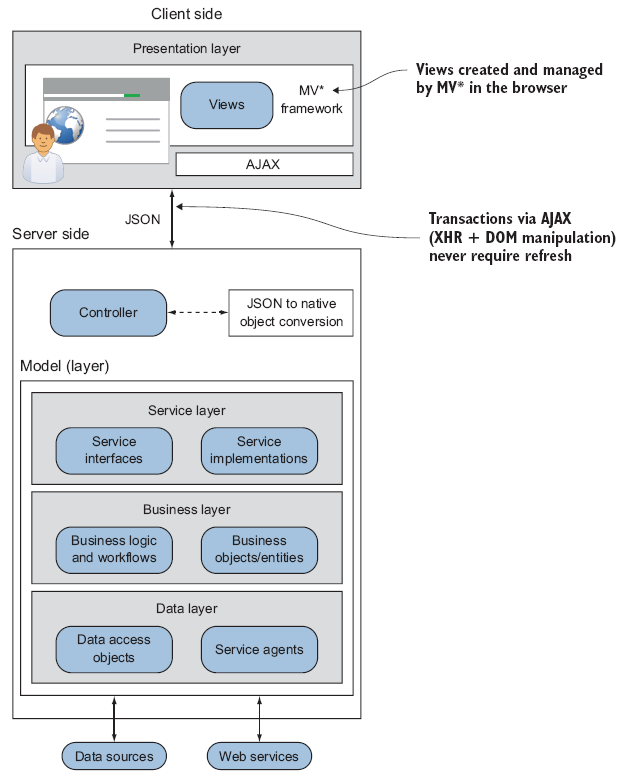
\includegraphics[scale=0.60]{images/Scott_SPA-overview.png}
    \caption[Aufbau einer \acs{SPA}]{Aufbau einer \acs{SPA}\newline(Quelle: \cite[][Seite 6]{scott_spa_2015})}
    \label{fig:spa-overview}
\end{figure}

\subsection{\acl{SSR}}
\label{subsec:ssr}
Neben der reinen Übertragung von Daten mittels \acs{JSON} (oder anderweitigen Datenformaten) kann bei \acsp{SPA} alternativ beziehungsweise erweiternd auch auf \ac{SSR} gesetzt werden. Bei diesem Ansatz werden Ausschnitte von HTML bereits auf dem Server vorbereitet und zusammen mit weiterführenden Daten an den Client geschickt. Dieser kann somit einen Teil der Antwort ohne weitere Aufbereitung darstellen, während die restlichen Daten mittels \ac{DOM}-Manipulation in die View eingebettet werden. \parencite[][Seite 7]{scott_spa_2015}

\subsection{Bestandteile einer \acs{SPA}}
\label{subsec:spa-bestandteile}
Der zugrundeliegende Aufbau einer \ac{SPA} - und der Bestandteil der Applikation, der lediglich einmal geladen wird - ist die sogenannte \textit{Shell}. Die Shell ist eine einzelne HTML-Datei, welche vom Browser vollständig geladen wird und in den meisten Fällen lediglich minimale Strukturen (ein Navigationsmenü, statische Inhalte etc.) sowie einen leeren \texttt{DIV} Tag enthält, wie Abbildung \ref{fig:spa-shell} auf Seite \pageref{fig:spa-overview} zeigt. Genutzt wird diese als Ausgangspunkt für alle weiteren Views, die unabhängig von der Shell agieren und dynamisch geladen werden. \parencite[][Seite 8]{scott_spa_2015}

\begin{figure}[ht]
    \centering
    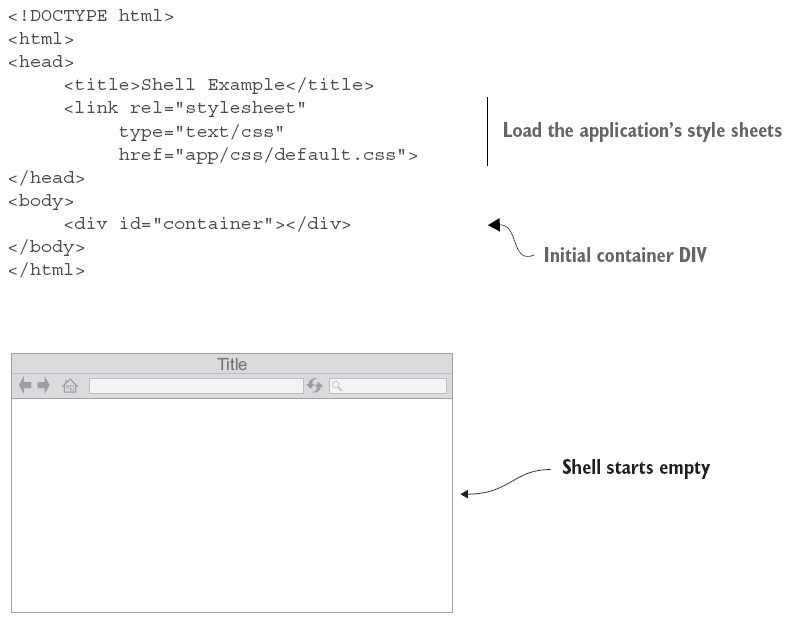
\includegraphics[scale=0.45]{images/Scott_SPA-shell.png}
    \caption[\acs{SPA} Shell]{\acs{SPA} Shell\newline(Quelle: \cite[][Seite 8]{scott_spa_2015})}
    \label{fig:spa-shell}
\end{figure}

Voneinander getrennt sichtbare Bereiche der Anwendung können im weiteren Verlauf ebenfalls mit \texttt{DIV} Tags abgegrenzt werden und sind dem in der Shell definierten \texttt{DIV} Container untergeordnet. Dies ermöglicht sowohl eine logische als auch inhaltliche Gruppierung und das gezielte Austauschen bestimmter Bereiche, sogenannter \textit{Regions}. \parencite[][Seite 9]{scott_spa_2015}

\medskip

Die einzeln dargestellten Views, welche dynamisch ausgetauscht werden können, stellen keine vollständigen HTML-Seiten dar, sondern bilden lediglich gezielt definierte Ausschnitte. Diese Ausschnitte werden bei jedem Navigationsvorgang innerhalb der Website durch das entsprechend eingesetzte Framework ausgetauscht und erfordern kein erneutes Laden der Website. \parencite[][Seite 10f.]{scott_spa_2015}

\section{Vorteile einer \acs{SPA} gegenüber einer \acs{MPA}}
\label{sec:vorteile-spa-mpa}
Der Einsatz und die Entwicklung einer \ac{SPA} bietet sowohl Vorteile für Entwickler:innen als auch Anwender:innen gegenüber der Nutzung einer klassischen \ac{MPA}.

Der bereits mehrfach angesprochene Vorgang, lediglich bestimmte Teile beziehungsweise Views der Webanwendung auszutauschen, erhöht die Benutzbarkeit sowie die \ac{UX} laut Mikowski und Powell deutlich. Da keine komplett neue (Unter-)Seite geladen werden muss, entfällt das Aufscheinen einer - abhängig von der Internet- und Servergeschwindigkeit - kurz sichtbaren, weißen Übergangsseite während des Ladeprozesses. Dem:Der Benutzer:in kann stattdessen beispielsweise ein dynamisch dargestellter Fortschrittsbalken dargestellt werden, der sich bei vorhandener Ladezeit laufend aktualisiert. \parencite[][Seite 20]{mikowski_single_2013}

Scott hebt hervor, dass die Aufteilung in eine entkoppelte Präsentationsschicht auf dem Client dazu führt, dass diese unabhängig von der Logik auf dem Server gewartet und aktualisiert werden kann. Während bei klassischen \acsp{MPA} stellenweise HTML, JavaScript etc. mit serverseitigem Code (beispielsweise \textit{PHP}, \textit{JavaServer Pages}, ...) vermischt werden, kann bei \acsp{SPA} zudem eine gewisse Differenzierung und Abtrennung von HTML, CSS und JavaScript im Frontend erzielt werden, was die Wartbarkeit ebenfalls erhöht. \parencite[][Seite 13]{scott_spa_2015}

\newpage

Sowohl Mikowski und Powell als auch Scott gehen des Weiteren darauf ein, dass die Datenübertragung und Verarbeitung bei einer \ac{SPA} effizienter und schneller stattfinden kann, als bei einer \ac{MPA}. Die Programmlogik zur Darstellung und dynamischen Entscheidungsfindung befindet sich beim Client (weshalb dieser Operationen schnell durchführen kann), während der Server lediglich Validierung, Authentifizierung und Datenspeicherung durchführt. \parencite[][Seite 20]{mikowski_single_2013} Zudem sind Transaktionen zwischen Client und Server nach dem Initialen Aufruf der Applikation schneller, da lediglich Daten in einem vorab definierten Datenformat asynchron übertragen und keine kompletten HTML-Seiten samt JavaScript und CSS ausgetauscht werden müssen. \parencite[][Seite 13]{scott_spa_2015}

\section{Funktionsweise von Vaadin}
\label{sec:funktionsweise-angular-vaadin}
Sowohl Angular als auch Vaadin sind beides Frameworks, die das Entwickeln von \acp{SPA} unterstützen und ermöglichen. Der gewählte Ansatz, die zugrundeliegenden Technologien und die jeweiligen Herangehensweisen unterscheiden sich stellenweise jedoch deutlich voneinander.

Der nachfolgende Abschnitt befasst sich daher im Detail mit der Funktionsweise und den Konzepten von Vaadin sowohl aus dem Blickwinkel von Entwickler:innen als auch Anwender:innen. Wo sinnvoll, wird ein direkter Vergleich zu Angular gezogen und darauf eingegangen, wie die beiden Frameworks Probleme unterschiedlich handhaben und lösen.

\subsection{Ansätze von Vaadin}
\label{sub-sec:vaadin-ansaetze}
Vaadin ist ein Framework beziehungsweise eine Plattform, mit der Webapplikationen sowohl komplett in Java, vollständig mit TypeScript und HTML als auch in einer Kombination beider entwickelt und umgesetzt werden können. Die beiden Ansätze sind dabei in zwei verschiedene Frameworks aufgeteilt, um - je nach Einsatzzweck - diese entsprechend einzusetzen:

\begin{itemize}
    \item \textbf{Vaadin Flow} ist ein Framework, mit dem Webapplikationen in Java umgesetzt werden können. Technologien wie beispielsweise HTML oder JavaScript werden bei der Entwicklung der \acs{UI} nicht benötigt, der gesamte Programmcode basiert auf einer einheitlichen Programmiersprache. Die gesamte Anwendung selbst läuft auf einem Server, während das Framework den Applikationszustand sowie die Client-Server-Kommunikation übernimmt.  \parencite[][]{vaadin_ltd_vaadin_nodate}
    \item \textbf{Vaadin Fusion} ist ein Framework, bei dem TypeScript für das Frontend auf dem Client und Java für das Backend auf dem Server eingesetzt wird. Mit Fusion können clientseitig reaktive Webapplikationen entwickelt werden, die typsichere Java Endpunkte aufrufen. Vorgefertigte Komponenten erleichtern hierbei das Entwickeln der \acs{UI}, während eigene Elemente mittels voller Kontrolle über das \ac{DOM} umgesetzt werden können. \parencite[][]{vaadin_ltd_vaadin_nodate-1}
\end{itemize}

Diese Arbeit befasst sich nachfolgend primär mit \textit{Vaadin Flow}, um eine alternative Herangehensweise aufzuzeigen, wie eine \ac{SPA} komplett auf dem Server und mittels Java entwickelt werden kann. Durch diesen Fokus kann im weiteren Verlauf ein tiefergehenderer Vergleich der Funktionalitäten und Konzepte von Vaadin und Angular bewerkstelligt werden, der bei spezifischen Punkten konkret auf die Unterschiede der beiden Technologien eingeht.

\subsection{Frontend und Backend in Java}
\label{sub-sec:frontend-backend-java}
Vaadin selbst schreibt, dass sich das Arbeiten mit HTML, CSS und JavaScript für reine Java-Entwickler sowohl als herausfordernd als auch als zeitintensiv darstellt. \parencite[][Framework - Introduction - Overview]{vaadin_ltd_documentation_nodate}

Vaadin Flow bietet daher die Möglichkeit, mit einer vollständig in Java geschriebenen Applikation - die auf einem Server ausfgeführt wird - jeweils die Anwendungslogik sowie das \acl{UI} umzusetzen. Die Vielzahl von sogenannten \textit{Components}, welche Vaadin von Haus aus mitliefert und einzelnen Bestandteilen wie beispielsweise einem Button oder ähnlichem entspricht, unterstützen Entwickler:innen dabei, bei Bedarf ohne HTML oder JavaScript auszukommen. Die Components steuern dabei das zugrundeliegende JavaScript im Hintergrund über die Framework-eigene \textit{Java API} beziehungsweise die \textit{Java Component API}. Der Quellcode \ref{code:vaadin-ui-java-sample} auf Seite \pageref{code:vaadin-ui-java-sample} stellt einen stark vereinfachten Ausschnitt von Components dar, die so im Client bereits entsprechend dargestellt werden. \parencite[][Framework - Introduction - Overview]{vaadin_ltd_documentation_nodate}

\begin{listing}[ht]
    \inputminted[fontsize=\footnotesize,linenos]{java}{code/Vaadin_Java-UI-sample.java}
    \caption[Beispiel einer einfachen \acs{UI} mittels der \textit{Java API}]{Beispiel einer einfachen \acs{UI} mittels der \textit{Java API}\newline(Quelle: \cite[][]{vaadin_ltd_overview_2021})}
    \label{code:vaadin-ui-java-sample}
\end{listing}

Während mit Vaadin Flow hauptsächlich in Java, und somit auf dem Server, entwickelt wird, bietet das Framework dennoch die Möglichkeit, auf Browser \acsp{API}, spezifische Web Components sowie auf das \ac{DOM} zuzugreifen.

Als Vorteil stellt sich zudem heraus, dass die Anbindung des Frontends an ein Backend in den meisten Fällen mit Vaadin Flow bereits komplett vorhanden ist und nicht separat mit auf REST basierender Kommunikation umgesetzt werden muss. Dadurch kann die \acs{UI} und die dafür benötigten Daten direkt über Java verknüpft und auch aktualisiert werden. Hierbei unterstützen mitgelieferte \textit{Events} und \textit{Event Listener} die Entwicklung und Benutzbarkeit, indem Änderungen auf dem Client automatisch auch auf dem Server - und umgekehrt - abgebildet werden. \parencite[][]{vaadin_ltd_overview_2021-2}

\subsection{Kommunikation zwischen Client und Server}
\label{sub-sec:kommunikation-client-server}
Bei einer \ac{SPA} spielt die Kommunikation des Clients (dem JavaScript/TypeScript Frontend) und dem Server (dem Backend) eine sehr wichtige Rolle. Im Gegensatz zu \acp{MPA}, bei denen die Daten bereits auf dem Server verarbeitet, eingebettet und als Ganzes übertragen werden, werden bei \acsp{SPA} diese erst bei Bedarf und im Nachhinein geladen. Die Art und Weise, wie dieser Vorgang umgesetzt wird, unterscheidet sich bei Vaadin Flow und Angular jedoch deutlich voneinander.

\subsubsection{Automatische Kommunikation von Vaadin}
\label{sub-sub-sec:kommunikation-herangehensweise-vaadin}
Da sowohl die Persitenzschicht, die Applikationslogik als auch das \acl{UI} bei Vaadin Flow mittels Java umgesetzt werden können, ergibt sich der Vorteil, dass die Kommunikation zwischen Client und Server vom Framework selbst übernommen wird und hierbei unter anderem auf das bereits angesprochene \textit{Two-way data binding} setzt. Die Nutzung von Vaadin-eigenen Components bietet des Weiteren die Möglichkeit, das \ac{DOM} im Webbrowser selbst zu steuern, während eine Repräsentation desselben \ac{DOM} serverseitig in Java gehalten wird. Änderungen, die auf dem Client durchgeführt werden, werden automatisch synchronisiert. \parencite[][Framework - Introduction - Core Concepts]{vaadin_ltd_documentation_nodate}

\medskip

Artur Signell, CTO der Vaadin Ltd., erklärt währenddessen in einem Foren-Beitrag vom Juni 2018, dass genauere Informationen zur tatsächlich Umsetzung der automatisch vorgenommen Kommunikation nicht nach außen kommuniziert werden, da die Umsetzung davon als rein internes Implementierungsdetail gehandhabt wird. \parencite[][]{signell_explanation_2018}

\medskip

Mittels den Entwicklertools, die in gängigen Webbrowsern zur Verfügung stehen, kann sich - abseits der nicht vorhandenen Dokumentation - jedoch ein kurzes Bild davon gemacht werden, wie die Kommunikation grundsätzlich funktioniert. Die Abbildung \ref{fig:vaadin-json-communication} auf Seite \pageref{fig:vaadin-json-communication} zeigt die vom Client an den Server geschickte Anfrage, die durch das Befüllen eines Vaadin \texttt{TextField} (einem HTML - \texttt{INPUT} Element) ausgelöst wird. Für die Kommunikation wird \acs{JSON} eingesetzt, welches die in das \texttt{INPUT} Element eingefüllten Daten mit gängiger HTTP-Kommunikation an den Server schickt, auf die schlussendlich mittels Java-typischer Notation zugegriffen werden kann.

\begin{figure}[ht]
    \centering
    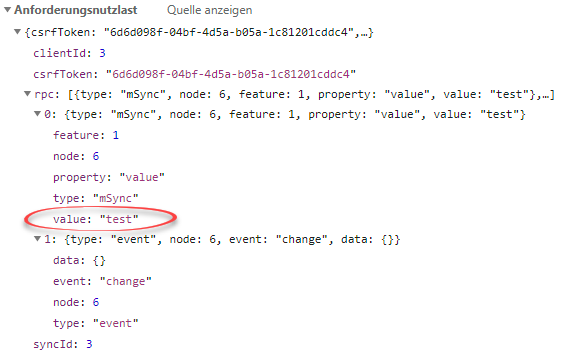
\includegraphics[scale=0.75]{images/Luidold_Vaadin-HTTP-communication.png}
    \caption[Automatisch erzeugte Kommunikation von Vaadin Flow]{Automatisch erzeugte Kommunikation von Vaadin Flow\newline(Quelle: eigene Abbildung)}
    \label{fig:vaadin-json-communication}
\end{figure}

\newpage

\subsubsection{Anpassbare Kommunikation bei Angular}
\label{sub-sub-sec:kommunikation-herangehensweise-angular}
Im Vergleich zur automatischen Kommunikation, die Vaadin Flow von Haus aus bietet, unterstützt Angular Entwickler:innen zwar beim Datenaustausch mit einem Server, die konkrete Umsetzung muss jedoch deutlich eigenständiger programmiert werden.

\medskip

Der von Angular entwickelte \texttt{HttpClient} Service - der über das \path{@angular/common/http} Package bezogen werden kann - stellt eine entsprechende API zur Verfügung, mit der typisierte \texttt{Response} Objekte angefordert werden können, eine vereinheitlichte Fehlerbehandlung ermöglicht wird sowie das Abfangen und Bearbeiten von \texttt{Request} und \texttt{Response} Objekten erlaubt. \parencite[][]{google_llc_communicating_nodate}

\medskip

Der Einsatz der angesprochenen API kann bei Angular grundsätzlich im gesamten Projekt erfolgen, Wilken empfiehlt jedoch, die Nutzung von der tatsächlichen Logik zu abstrahieren und dafür einen eigenständigen Service zu erstellen. Der \texttt{HttpClient}, welcher zur Kommunikation mit einem Server (und gegebenenfalls in einem eigenständigen Service) verwendet wird, unterstützt HTTP Request-Methoden wie beispielsweise \texttt{GET}, \texttt{POST}, \texttt{PUT} und \texttt{DELETE}, die bei einem entsprechenden Aufruf ein \texttt{Observable} als Antwort liefern. Mit diesem kann in weiterer Folge in der Applikation gearbeitet und auf die Daten zugegriffen werden. \parencite[][Seite 142-144.]{wilken_angular_2018}

\medskip

Der Quellcode \ref{code:angular-sample-httpclient-service} auf Seite \pageref{code:angular-sample-httpclient-service} zeigt einen exemplarischen Service, der mittels \texttt{HTTP GET} eine Anfrage an den Server beziehungsweise einen API Endpunkt stellt und ein Array des Typs \texttt{Sample} als Antwort zurückliefert.

\begin{listing}[ht]
    \renewcommand{\fcolorbox}[4][]{#4}
    \inputminted[fontsize=\footnotesize,linenos]{js}{code/Luidold_HttpClient-Service.ts}
    \caption[Exemplarische Nutzung des \texttt{HttpClient} in einem Service]{Exemplarische Nutzung des \texttt{HttpClient} in einem Service}
    \label{code:angular-sample-httpclient-service}
\end{listing}

Der Quellcode \ref{code:angular-sample-data-function} auf Seite \pageref{code:angular-sample-data-function} zeigt in Folge die Nutzung der gerade eben demonstrierten Funktion, bei der die Daten mittels \texttt{subscribe()} abgefragt werden können und entsprechend zugewiesen werden, sobald diese zur Verfügung stehen.

\begin{listing}[ht]
    \renewcommand{\fcolorbox}[4][]{#4}
    \inputminted[fontsize=\footnotesize,linenos]{js}{code/Luidold_Load-function.ts}
    \caption[Beispielhafte Nutzung der \texttt{getSampleData} Funktion]{Beispielhafte Nutzung der \texttt{getSampleData} Funktion}
    \label{code:angular-sample-data-function}
\end{listing}

Verglichen mit der im Abschnitt \ref{sub-sub-sec:kommunikation-herangehensweise-vaadin} auf Seite \pageref{sub-sub-sec:kommunikation-herangehensweise-vaadin} beschriebenen Herangehensweise von Vaadin unterscheidet sich Angular deutlich. Wilken merkt an, dass die Nutzung des \texttt{HttpClient} der am häufigsten verwendete Ansatz bei Angular darstellt. Um eine Kommunikation mit einem Server herzustellen, können laut ihm jedoch auch, beziehungsweise zusätzlich, diverse andere Protokolle und Technologien genutzt werden. \parencite[][]{wilken_angular_2018}

\subsection{Vaadin Components und deren Grundlage}
\label{sub-sec:vaadin-components}
\textit{Vaadin Components} sind von Vaadin entwickelte \enquote{\acs{UI}-Module}, die zur einfachen Entwicklung von gängigen \acl{UI} Bestandteilen genutzt werden können. Diese sind bereits im Vaadin Framework enthalten, können im Zuge der Nutzung der Web Components Technologien jedoch unabhängig von Vaadin selbst und somit in allen gängigen Applikationen sowie Webbrowsern genutzt werden. \parencite[][Seite 2ff.]{vaadin_ltd_vaadin_nodate-2}

Die Abbildung \ref{fig:vaadin-components-overview} auf Seite \pageref{fig:vaadin-components-overview} zeigt hierbei eine Auswahl von Vaadin Components, die häufig in Webapplikationen genutzt werden und entsprechend für das Framework umgesetzt wurden.

\begin{figure}[ht]
    \centering
    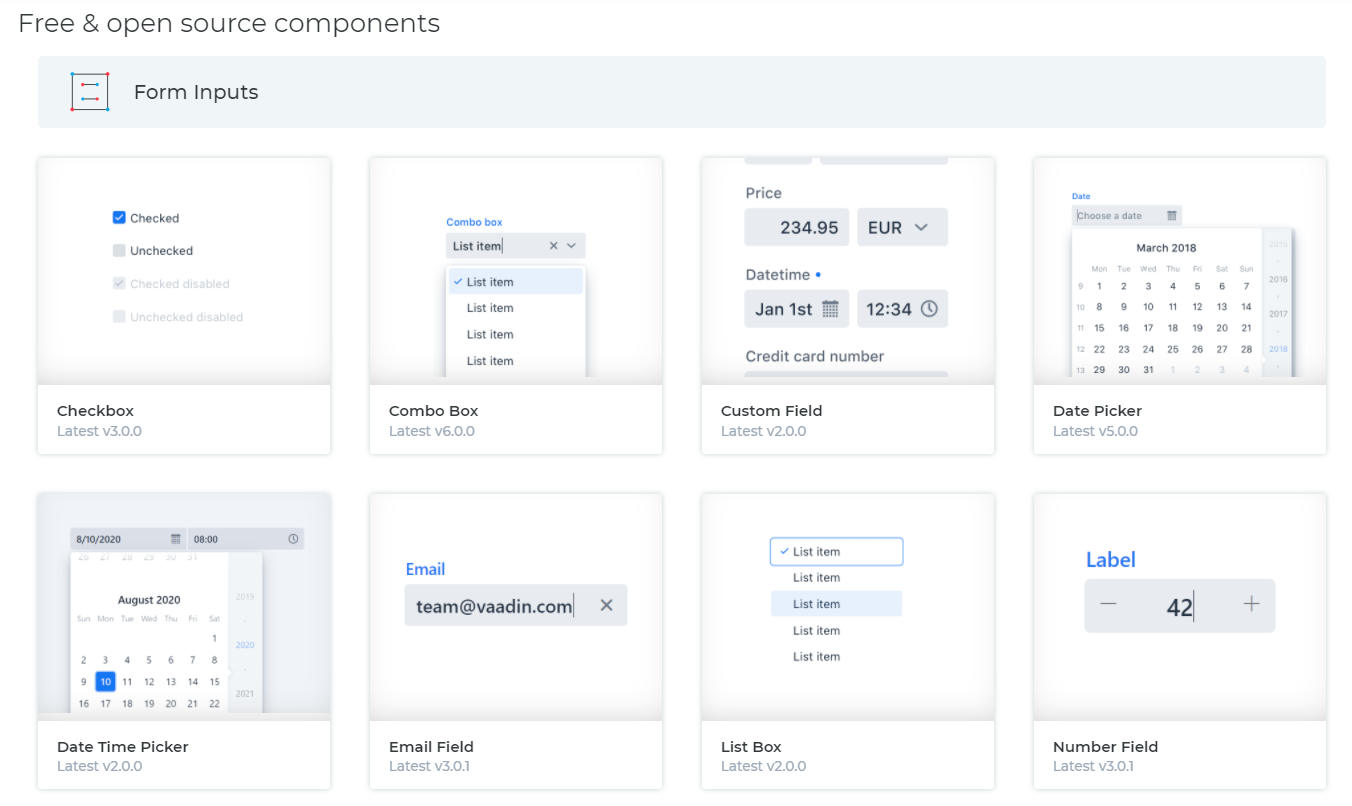
\includegraphics[scale=0.38]{images/Vaadin_Components-overview.png}
    \caption[Auswahl von Open Source Vaadin Components]{Auswahl von Open Source Vaadin Components\newline(Quelle: \cite[][]{vaadin_ltd_mobile_nodate})}
    \label{fig:vaadin-components-overview}
\end{figure}

Die Technologien, auf die sich Vaadin bei der Implementierung und Umsetzung der Components stützt, bauen auf diversen Konzepten auf, zu denen unter anderem \textit{Custom elements}, \textit{Shadow \ac{DOM}} sowie \textit{HTML templates} gehören. Diese werden dazu genutzt, um mittels JavaScript spezifische Klassen für die gewünschten, neuen Web Components zu erstellen, diese entsprechend zu registrieren und mittels Template-Funktionalität die neu erstellten Objekte schlussendlich zu definieren. \parencite[][]{mozilla_contributors_web_2021}

\medskip

Der Quellcode \ref{code:mozilla-sample-web-component} auf Seite \pageref{code:mozilla-sample-web-component} zeigt beispielhaft auf, wie der grundlegende Aufbau eines eigens umgesetzten Web Components aussieht. Vaadin nutzt diesen Aufbau sowie die zugrundeliegende Herangehensweise für die Umsetzung der vorhergehend aufgezeigten \textit{Vaadin Components}. \parencite[vgl.][]{vaadin_ltd_vaadin-text-fieldjs_2021} Aufgrund des Fokus dieser Arbeit wird im weiteren Verlauf jedoch nicht näher auf die zugrundeliegende Struktur von Web Components eingegangen.

\begin{listing}[ht]
    \inputminted[fontsize=\footnotesize,linenos]{js}{code/Mozilla_Web-Component-sample.js}
    \caption[Beispiel für den grundlegenden Aufbau eines eigenen Web Components]{Beispiel für den grundlegenden Aufbau eines eigenen Web Components (Quelle: \cite[][]{mozilla_contributors_using_2021})}
    \label{code:mozilla-sample-web-component}
\end{listing}

Die Nutzung der Vaadin Components lässt sich sowohl eigenständig mit anderen Frameworks als auch direkt in Vaadin selbst mittels der sogenannten \textit{Java API} umsetzen. Jede Komponente besitzt beim Einsatz von Java entsprechende Objekt-Typen und dazugehörige Attribute, bei der Verwendung von HTML stehen Tags mit ähnlicher Funktionalität zur Verfügung. \parencite[][]{vaadin_ltd_mobile_nodate}

\medskip

Quellcode \ref{code:vaadin-textfield} auf Seite \pageref{code:vaadin-textfield} ermöglicht einen Einblick, wie ein \textit{Text Field} Component mittels Vaadins Java API genutzt werden kann. Die deklarierten und initialisierten \texttt{TextField} Objekte können, in Java typischer Weise, an beliebiger Stelle genutzt werden. Weiterführende beziehungsweise benötigte Funktionalitäten können im Anschluss über das Zuweisen und Setzen von spezifischen Attributen erzielt werden, die das Verhalten des Textfeldes beeinflussen und vorgeben.

\begin{listing}[ht]
    \inputminted[fontsize=\footnotesize,linenos]{java}{code/Vaadin_Text-Field_sample.java}
    \caption[Mögliche Umsetzungen des Vaadin \textit{Text Field}]{Mögliche Umsetzungen des Vaadin \textit{Text Field}\newline(Quelle: \cite[][Basic text field]{vaadin_ltd_java_nodate})}
    \label{code:vaadin-textfield}
\end{listing}

Abbildung \ref{fig:vaadin-textfield-output} auf Seite \pageref{fig:vaadin-textfield-output} bezieht sich maßgeblich auf Quellcode \ref{code:vaadin-textfield}, da die dargestellten Textfelder jene sind, die mittels der aufgezeigten \texttt{TextField} Objekte erzeugt wurden und mittels gesetzter Attribute unterschiedliche Ausgangspunkte liefern.

\begin{figure}[ht]
    \centering
    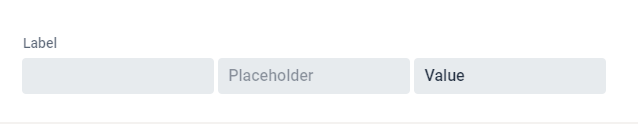
\includegraphics[scale=0.7]{images/Vaadin_Text-Field-output.png}
    \caption[Erzeugter Output von Quellcode \ref{code:vaadin-textfield}]{Erzeugter Output von Quellcode \ref{code:vaadin-textfield}\newline(Quelle: \cite[][Basic text field]{vaadin_ltd_java_nodate})}
    \label{fig:vaadin-textfield-output}
\end{figure}

\subsection{Routing und Navigation}
\label{sub-sec:routing-navigation}
Wilken schreibt, dass die meisten Webapplikationen die Funktionalität benötigen, während der Nutzung zwischen verschiedenen Seiten und Unterseiten navigieren zu können. \acp{MPA} laden beim Aufruf einer Seite die hinterlegten HTML, CSS und JavaScript Dateien von einem Webserver und nutzen dafür die angegebene URL. \acp{SPA} hingegen laden Daten asynchron und bei Bedarf und wechseln lediglich sogenannte Views und keine kompletten Seiten. Die Navigation innerhalb einer \ac{SPA} muss entsprechend anderweitig vorgenommen werden, wobei hier sowohl JavaScript an sich als auch das verwendete Framework eine wichtige Rolle spielt. \parencite[][Seite 159f.]{wilken_angular_2018}

\subsubsection{Routing bei Vaadin}
\label{sub-sub-sec:routing-herangehensweise-vaadin}
Vaadin bietet die Möglichkeit, mittels der \texttt{@Route} Annotation alle Components (sowohl Vaadin Components als auch eigene) über eine spezifische URL ansprechbar zu machen und diese somit aufrufen zu können. Quellcode \ref{code:route-annotation-vaadin} auf Seite    \pageref{code:route-annotation-vaadin} stellt beispielhaft dar, wie eine selbst entwickelte Komponente im Browser über die URL \path{http://example.com/some/path} angesteuert werden kann. \parencite[][Using the @Route Annotation]{vaadin_ltd_overview_2021-1}

\begin{listing}[ht]
    \inputminted[fontsize=\footnotesize,linenos]{java}{code/Vaadin_Route-annotation.java}
    \caption[Beispielhafte Nutzung der \texttt{@Route} Annotation]{Beispielhafte Nutzung der \texttt{@Route} Annotation\newline(Quelle: \cite[][Using the @Route Annotation]{vaadin_ltd_overview_2021-1})}
    \label{code:route-annotation-vaadin}
\end{listing}

Mittels verschiedener Events, die während der Nutzung der Webapplikation und der darin auftretenden Navigation ausgelöst werden, entsteht ein sogenannter \textit{Navigation Lifecycle}. Dieser kann dafür genutzt werden, um zusätzliche Funktionalitäten anzubieten. UI Komponenten implementieren dafür entsprechende \texttt{Listener}, welche auf zugehörigen \texttt{Observer} Interfaces aufbauen. Mit dem Navigation Lifecycle und einem \texttt{BeforeLeaveEvent} kann beispielsweise eine Abfrage im \acl{UI} erstellt werden, die Nutzer:innen bestätigen lässt, dass das Verlassen der Website womöglich zum Verlust von Daten führt. \parencite[][]{vaadin_ltd_navigation_2021}

\newpage

URL Parameter (sowohl solche, die Teil der URL selbst sind als auch Query Parameter) können mittels dem \texttt{HasUrlParameter} Interface abgefragt und im weiteren Verlauf genutzt werden. Wie Quellcode \ref{code:url-params-vaadin} auf Seite \pageref{code:url-params-vaadin} zeigt, kann über die \texttt{setParameter} Methode auf Teile der URL zugegriffen werden, die mittels Generics direkt in der Methode verankert sind. \parencite[][]{vaadin_ltd_typed_2021} Query Parameter lassen sich währenddessen mit dem \texttt{BeforeEvent} ebenfalls in derselben Methode abfragen. \parencite[][]{vaadin_ltd_query_2021}

\begin{listing}[ht]
    \inputminted[fontsize=\footnotesize,linenos]{java}{code/Luidold_Vaadin-URL-params.java}
    \caption[Zugriff auf URL Parameter bei Vaadin]{Zugriff auf URL Parameter bei Vaadin}
    \label{code:url-params-vaadin}
\end{listing}

\smallskip

Um die Navigation zwischen verschiedenen Routen zu ermöglichen, bietet Vaadin - neben dem händischen Abändern der URL im Browser - verschiedene Ansätze:

\begin{itemize}
    \item Mittels der \texttt{RouterLink} Komponente können Links erstellt werden, welche die angegebene Route als Ziel haben (\texttt{menu.add(new RouterLink("Home", HomeView.class));}). \parencite[][Using the RouterLink Component]{vaadin_ltd_navigating_2021}
    \item Gewöhnliche HTML Anker Tags können genutzt werden, um zwischen verschiedenen Routen zu navigieren (\texttt{<a href="company" [...]}). Diese verursachen jedoch ein Neuladen der gesamten Seite. Wenn der zusätzliche Ladeprozess der Seite verhindert werden soll, kann das Vaadin-eigene \texttt{router-link} Attribut zusätzlich angehängt werden. \parencite[][Using Standard href Links]{vaadin_ltd_navigating_2021}
    \item Serverseitig kann mittels \texttt{UI.navigate(/* Route name */)} der Wechsel zu einer neuen Route ausgelöst werden. \parencite[][Server-side Navigation]{vaadin_ltd_navigating_2021}
\end{itemize}

\subsubsection{Routing bei Angular}
\label{sub-sub-sec:routing-herangehensweise-angular}
Um bei Angular eine vergleichbare Routing und Navigation Funktionalität zu erzielen, wird das \path{@angular/router} Package benötigt, welches in das Projekt eingebunden werden muss. Anders als bei Vaadin können bei Angular Routen an zentraler Stelle definiert werden, bei denen angegeben wird, welche TypeScript Komponente für die Abhandlung zuständig ist, wie Quellcode \ref{code:angular-route-definition} auf Seite \pageref{code:angular-route-definition} zeigt. \parencite[][]{google_llc_angular_nodate}

\begin{listing}[ht]
    \inputminted[fontsize=\footnotesize,linenos]{js}{code/Angular_Routes-definition.js}
    \caption[Definition von Routen bei Angular]{Definition von Routen bei Angular\newline(Quelle: \cite[][]{google_llc_angular_nodate})}
    \label{code:angular-route-definition}
\end{listing}

Vom Prinzip her ähnlich bietet Angular ebenfalls die Möglichkeit, auf die in der URL enthaltenen Parameter zuzugreifen und in der Präsentations- sowie Applikationslogik zu verwenden. Hierfür wird das \texttt{ActivatedRoute} Objekt dem Konstruktor einer Komponente übergeben, welches sowohl den Zugriff auf die Query Parameter (\texttt{ActivatedRoute\#queryParams}) als auch Parameter, die Bestandteil der URL sind (\texttt{ActivatedRoute\#paramMap}), ermöglicht. Zudem stehen allgemeine Informationen zur Route selbst zur Verfügung. \parencite[][]{google_llc_angular_nodate}

\medskip

Links innerhalb der \acs{UI} werden - vergleichbar mit Vaadin - ebenso mit HTML Anker Tags und einem eigens dafür vorgesehenen Attribut erzeugt, beinhalten im Zuge der entsprechenden Darstellungsoptionen jedoch noch weitere Funktionalitäten. Quellcode \ref{code:angular-route-linking} auf Seite \pageref{code:angular-route-linking} stellt diesen Ansatz dar und beinhaltet zudem in Zeile 19 das benötigte \texttt{<router-outlet>} Element, welches die ausgewählten und geladenen Routen im Browser darstellt. \parencite[][]{google_llc_angular_nodate}

\begin{listing}[ht]
    \inputminted[fontsize=\footnotesize,linenos]{html}{code/Angular_Routing-tags.html}
    \caption[Verlinken von Routen innerhalb von Angular]{Verlinken von Routen innerhalb von Angular\newline(Quelle: \cite[][]{google_llc_angular_nodate})}
    \label{code:angular-route-linking}
\end{listing}

\chapter{Methodik und Vorgehensweise}
\label{chap:methodik-Vorgehensweise}
Die in Kapitel \ref{chap:stand-technik} ab Seite \pageref{chap:stand-technik} behandelten Punkte befassen sich mit den grundlegenden Konzepten einer \ac{SPA} und spezifischen Funktionalitäten sowie Herangehensweisen, auf denen Vaadin basiert. Wo sinnvoll, wurde zudem ein Vergleich zu Angular gezogen.

In den folgenden Kapiteln fokussiert sich diese Arbeit nun auf die Planung, Umsetzung und Beurteilung von zwei Demo-Applikationen, die auf denselben User Stories basieren, jedoch sowohl mit Vaadin als auch Angular umgesetzt werden. Ziel ist es, diese Webapplikationen entlang vorab definierter Kriterien zu entwickeln, um schlussendlich eine Bewertung durchführen zu können.

\section{Kriterien}
\label{sec:kriterien}
Die Kriterien, anhand derer sich die Umsetzung und Beurteilung richten werden, wurden bereits in der Einleitung im Abschnitt \ref{sec:zielsetzung} ab Seite \pageref{sec:zielsetzung} kurz aufgegriffen. Da diese jedoch noch nicht im Detail behandelt wurden, folgt in den nächsten Absätzen eine entsprechend genauere Darstellung.

\subsubsection*{Umsetzung als \acl{PWA}}
\label{sub-sec:kriterien-pwa}
Die Demo-Applikationen sollen in mehrerer Hinsicht als moderne Webapplikation genutzt werden können. Dazu gehört, neben der standardmäßigen Nutzung mittels gängiger Webbrowser auf dem Desktop, die Nutzung als \ac{PWA}, die vor allem für Smartphones optimiert und ausgelegt ist und sich ähnlich wie eine App verhält.

Bei der Umsetzung und Bewertung wird daher darauf eingegangen, in wie weit sich die Webanwendungen mit den von Vaadin und Angular zur Verfügung gestellten Mitteln als \acp{PWA} umsetzen lassen und welche Funktionalitäten schlussendlich zur Verfügung stehen.

\subsubsection*{Einsatz und Entwicklung eigener Web Components}
\label{sub-sec:kriterien-web-components}
In Abschnitt \ref{sub-sec:vaadin-components} wurde bereits auf die Vaadin eigenen \textit{Vaadin Components} eingegangen. Da die Wiederverwendbarkeit in der Entwicklung eine große Rolle spielt, und auch auf \acs{UI}-Komponenten zutrifft, sollen mehrfach verwendete Bestandteile der Demo-Applikationen mittels Web Components umgesetzt werden.

Bei der Umsetzung und Bewertung wird daher darauf eingegangen, in welchem Ausmaß die Frameworks die Umsetzung von Web Components - zusätzlich zu den gegebenen Browserstandards - unterstützen und ob sie den Entwicklungsprozess dabei erleichtern.

\subsubsection*{Lokale und serverseitige Datenanbindung/-haltung}
\label{sub-sec:kriterien-datenanbindung}
Eine \ac{SPA}, beziehungsweise Anwendungen allgemein, leben von den Daten, die sie verarbeiten und mit denen Nutzer:innen interagieren können. Gerade im Zuge der Umsetzung der Demo-Applikationen als \ac{PWA} stellt sich die Frage, wie Angular und Vaadin eine Datenanbindung und Datenhaltung lokal (sprich auf dem jeweiligen Endgerät) sowie auf einem Server ermöglichen.

Bei der Umsetzung und Bewertung wird daher darauf eingegangen, welche Möglichkeiten sich bieten, bei den entwickelten Anwendungen Daten sowohl lokal zu speichern (um beispielsweise eine Offline-Fähigkeit zu ermöglichen) und wie man diese an eine externe Datenbank auf einem Server anbinden kann.

\section{Vorgehensweise}
\label{sec:vorgehensweise}
Damit die Demo-Applikationen die eben genannten Kriterien beide gleichermaßen beinhalten und umsetzen, und somit bewertet werden können, werden diese in User Stories eingebettet. Die User Stories orientieren sich dabei jedoch an keinem vollständigen Applikations-Konzept, sondern zeigen verschiedene Anwendungsfälle auf, die in einem realen Umfeld ein Bewertungskriterium für die Auswahl eines Frameworks spielen können.

\subsection{User Stories}
\label{sub-sec:user-stories}
Nachfolgend sind zwei User Stories aufgelistet, die im Detail erklären, welche Funktionalitäten die Vaadin und Angular Demo-Applikation beinhalten sollen und die genannten Kriterien einfließen lassen.

\subsubsection*{User Story 1: Echtzeit Eingangskontrolle}
\label{sub-sec:user-story-1}

\paragraph*{Beschreibung:} Als Veranstalter:in einer Organisation möchte ich kommende und gehende Besucher:innen bei allen Ein-/Ausgängen in Echtzeit erfassen, sodass diese den Veranstaltungsort nur in kontrollierter Weise betreten können.

\paragraph*{Akzeptanzkriterien:}

\begin{itemize}
    \item Besucher:innen können aus einer vorhandenen Teilnehmer:innenliste ausgewählt werden, um festzulegen, ob sie sich innerhalb oder außerhalb vom Veranstaltungsort befinden.
    \item Wird der Status eine:r Besucher:in aktualisiert, wird diese Änderung automatisch auf allen Instanzen sichtbar, ohne dass man diese manuell neu laden muss. Entspricht Multi-Nutzer:innen-Fähigkeit.
    \item Die Anwendung wird sowohl auf Computern als auch im mobilen Einsatz auf einem gängigen Smartphone unterstützt.
    \item Wenn keine Internetverbindung vorhanden ist, ist zumindest der zuletzt verfügbare Stand der Besucher:innenliste aufrufbar.
\end{itemize}

\subsubsection*{User Story 2: Fotoverwaltung}
\label{sub-sec:user-story-2}

\paragraph*{Beschreibung:} Als Nutzer:in möchte ich meine Fotos hochladen können, sodass diese an einem zentralen Ort gespeichert sind und man jederzeit darauf zugreifen kann.

\paragraph*{Akzeptanzkriterien:}

\begin{itemize}
    \item Nutzer:innen können Fotos von ihrem Computer oder Smartphone auswählen und hochladen, damit diese in einer zentralen Galerie angesehen werden können.
    \item Wenn Fotos von einem anderen Client hochgeladen wurden, kann man diese mit dem aktuellen Gerät ebenso ansehen, ohne dieser erneut hochzuladen oder synchronisieren zu müssen.
    \item Wenn keine Internetverbindung vorhanden ist, werden Fotos lokal gespeichert und können hochgeladen werden, sobald wieder eine Verbindung zur Verfügung steht.
\end{itemize}

% Literaturverzeichnis:
\clearpage
\phantomsection
\addcontentsline{toc}{chapter}{Literaturverzeichnis}
\printbibliography

\chapter*{Eidesstattliche Erklärung}
\addcontentsline{toc}{chapter}{Eidesstattliche Erklärung}
Ich erkläre hiermit an Eides statt, dass ich die vorliegende Bachelorarbeit II selbstständig und ohne Benutzung anderer als der angegebenen Hilfsmittel angefertigt habe. Die aus fremden Quellen direkt oder indirekt übernommenen Stellen sind als solche kenntlich gemacht. Die Arbeit wurde bisher weder in gleicher noch in ähnlicher Form einer anderen Prüfungsbehörde vorgelegt und auch noch nicht veröffentlicht.

\vspace{5cm}
\noindent
Dornbirn, am \colorbox{yellow}{20. Mai 2021}\hfill Dominic Luidold

\end{document}
